%!TEX program = xelatex
\documentclass{beamer}

\usepackage{blindtext}

\usepackage{fontenc} % added by Aurelie Jean 

\usetheme{Execushares}

\definecolor{isvblue}{RGB}{37,5,247} % ISV blue color (#2505F7)

\linespread{1.5}

\title{CODE CHALLENGE!\\ write and code an Algorithm to average the online client reviews}
\subtitle{\textcolor{isvblue}{\textit{Coding for a brighter and better future for everyone}}}

\titlegraphic{}
    %
\includegraphics[width=0.30\textwidth]{./pictures/chanel.jpg}\hspace{5.0cm}
    %          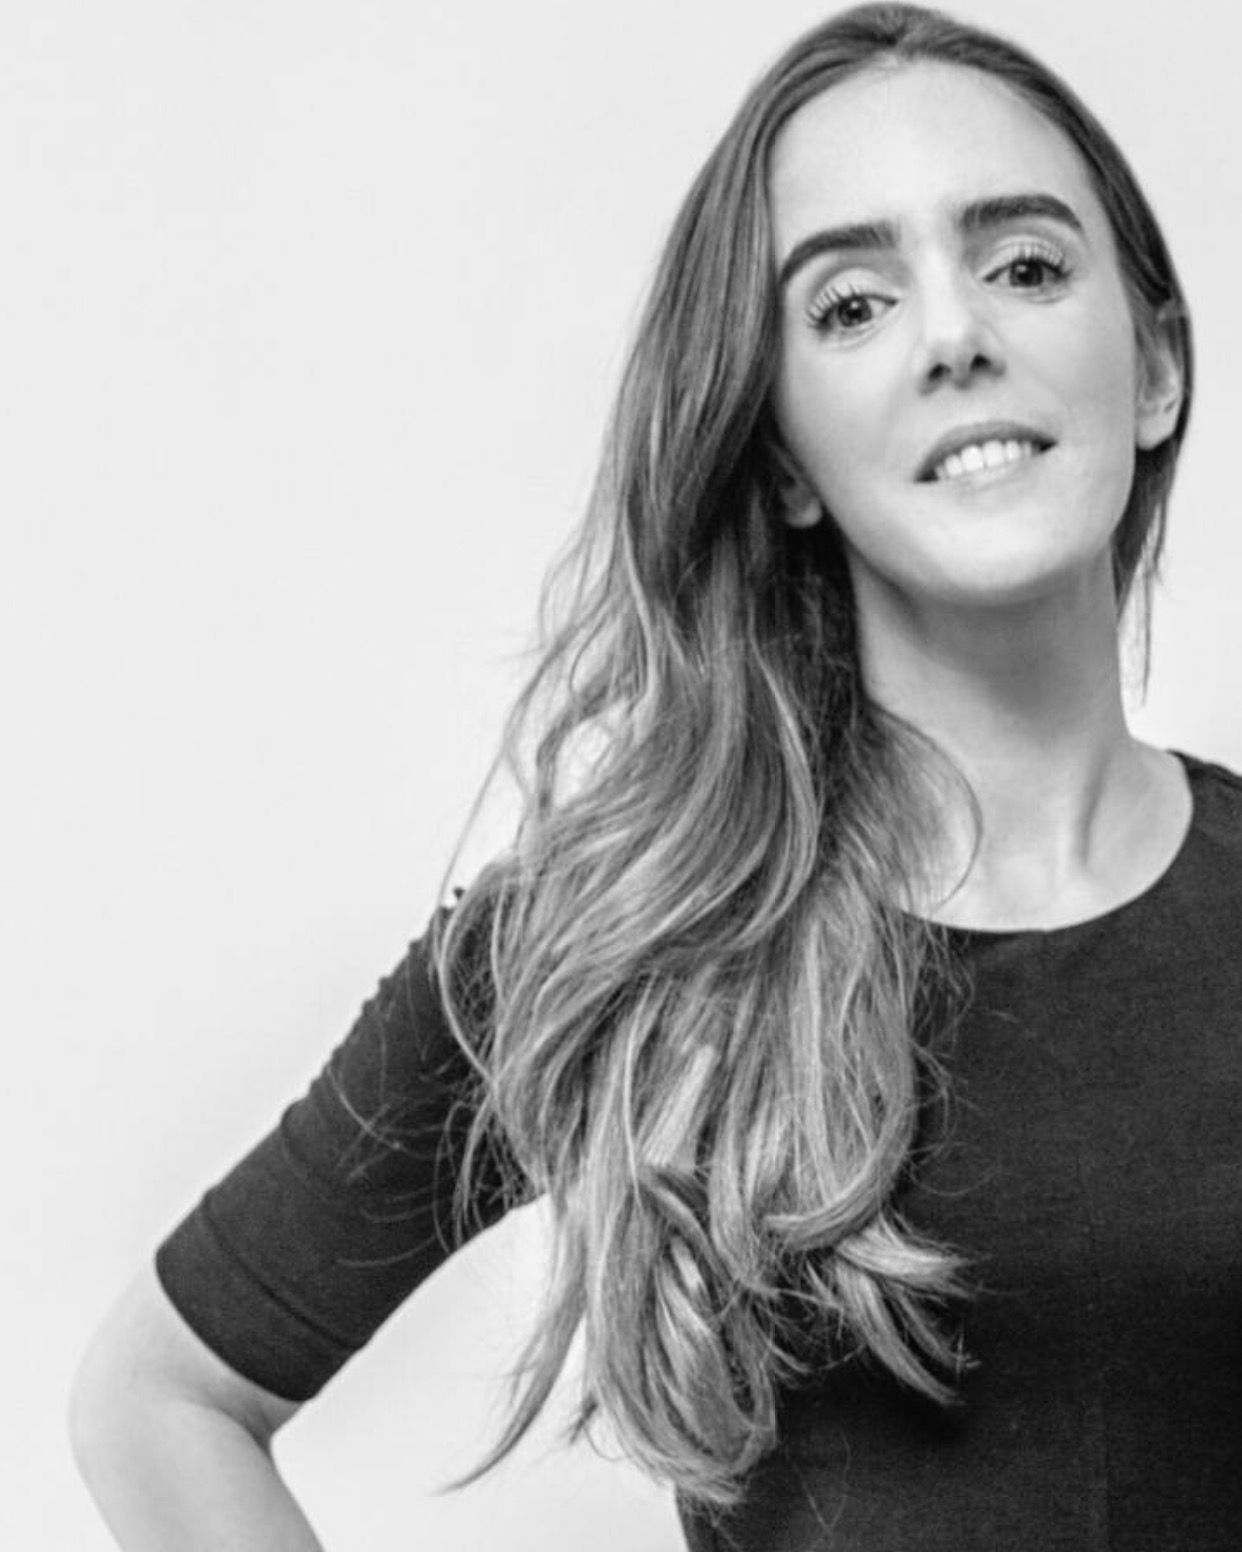
\includegraphics[width=0.26\textwidth]{./pictures/Aurelie-Jean_2016_001.JPG}}

\author{Aur\'elie JEAN and Alain BUZZACARO}
\institute{\textcolor{isvblue}{aurelie@silicoveritas.com - abuzzacaro@octo.com}}
\date{\#Coding4CLevels - January 10th and 11th 2018}

%\setcounter{showSlideNumbers}{1}

\begin{document}
	\setcounter{showProgressBar}{0}
	\setcounter{showSlideNumbers}{0}

        \begin{frame}%[label=pageone]
        \maketitle
        \end{frame}


	\setcounter{framenumber}{0}
	\setcounter{showProgressBar}{1}
	\setcounter{showSlideNumbers}{1}

        \section{Our Product}
        \begin{frame}
\frametitle{Our product: WinWin app from CoolCode}
\vskip 1.15cm
    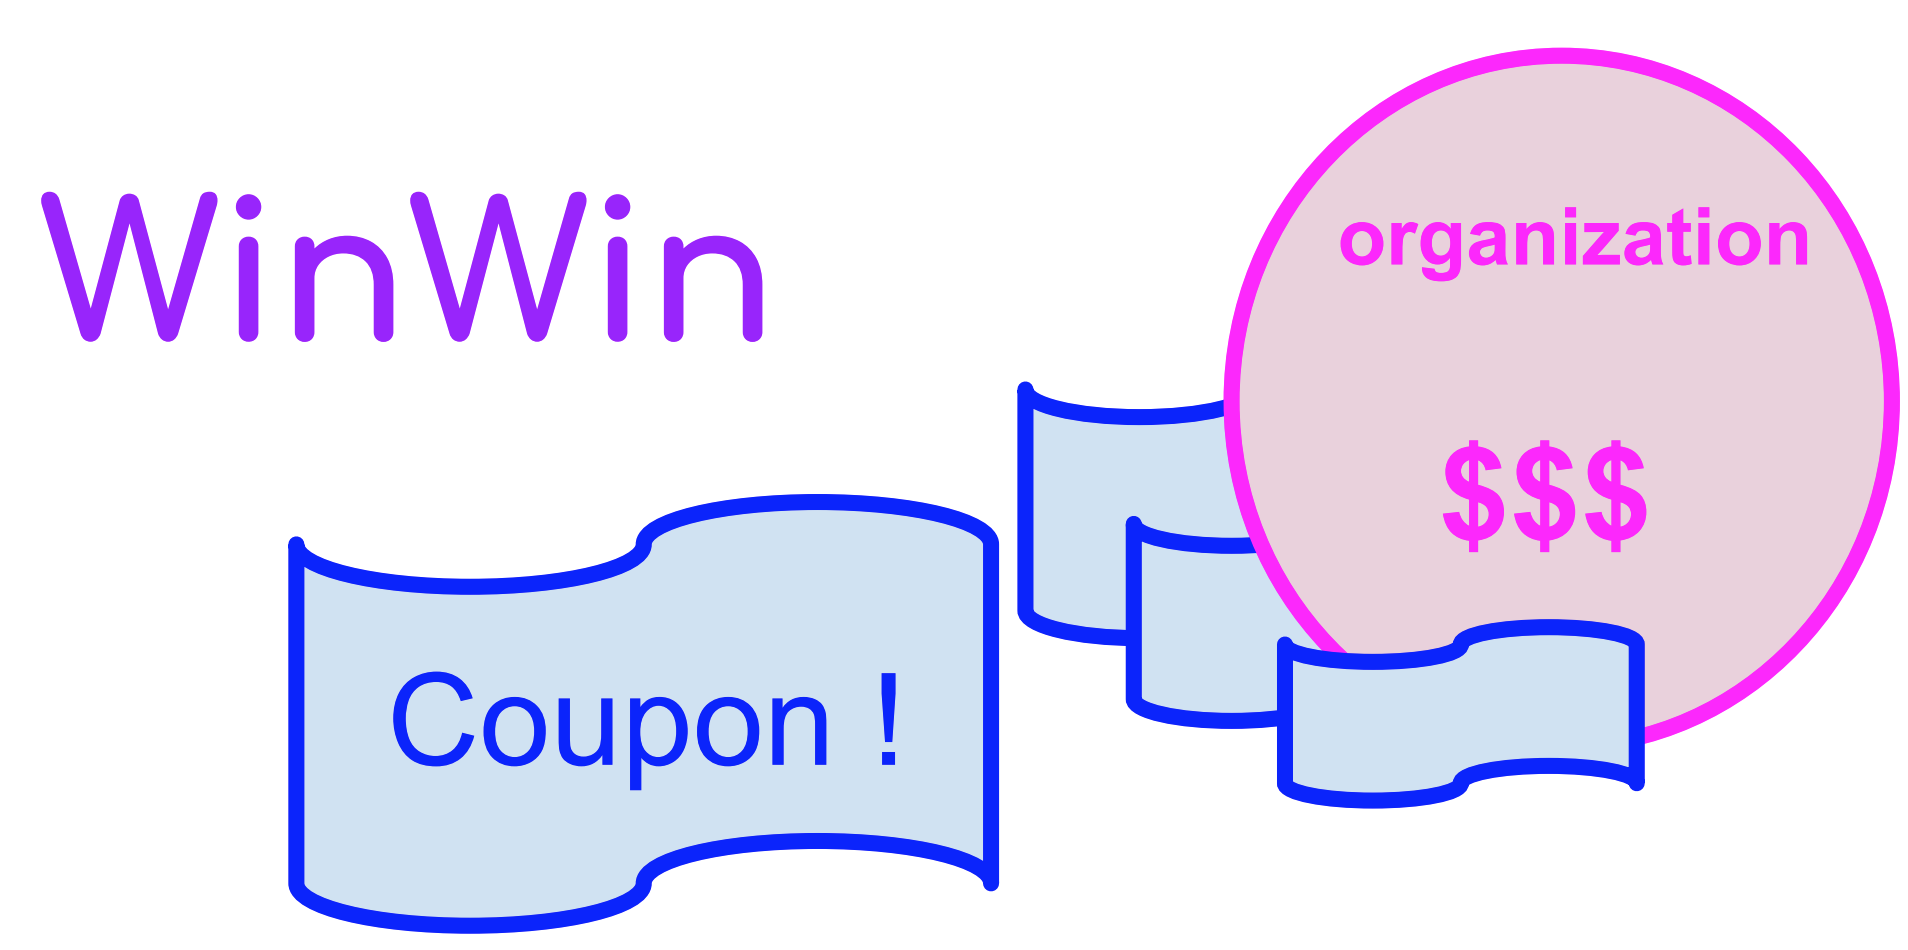
\includegraphics[width=1.0\textwidth]{./pictures/coupon-001.png}
\end{frame}




        \section{Our Goals and Challenges}
        \begin{frame}
\frametitle{Goals and Challenges}
\textcolor{isvblue}{\textbf{Goals:}}
\begin{itemize}    
  \item \textcolor{isvblue}{Compute} the average online client reviews
  \item \textcolor{isvblue}{Update} the average on real time
\end{itemize}    
\vskip 0.2cm
\visible<2->{\textcolor{isvblue}{\textbf{Challenges:}}
\begin{itemize}    
  \item \textcolor{isvblue}{Large amount} of data 
  \item \textcolor{isvblue}{Real time} computation
\end{itemize}}  
\vskip 0.4cm
\visible<3>{\textcolor{isvblue}{$\Rightarrow$ Write and Code an \textbf{Efficient Algorithm}}} 
\end{frame}



        \section{Efficient Algorithm?}
        \begin{frame}
\frametitle{Efficient Algorithm?}
\vskip 1.0cm
    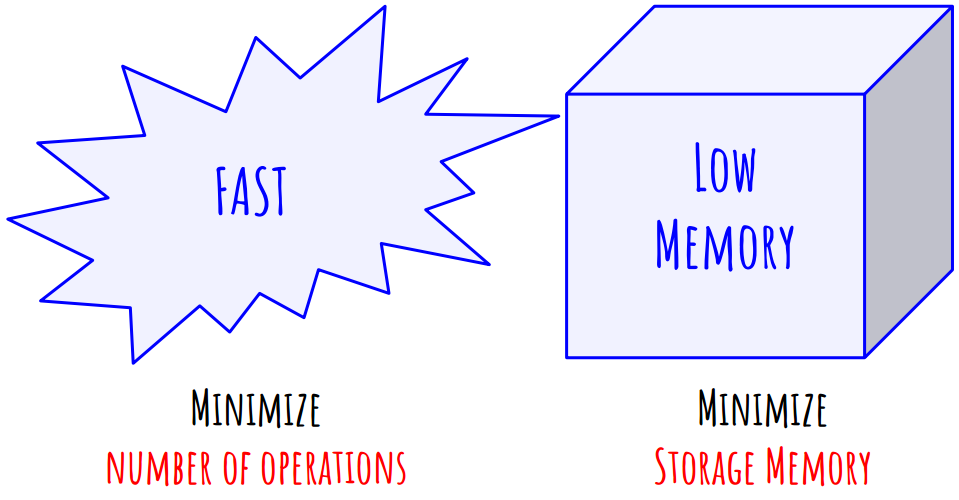
\includegraphics[width=1.0\textwidth]{./pictures/efficient.png}
\end{frame}

\begin{frame}
\frametitle{An example: simple average}
\vskip 0.6cm
\visible<2->{When measuring the average over \textcolor{isvblue}{2 reviews}:}
\begin{center}
    \visible<3->{$Average = \displaystyle{\frac{R_{1} + R_{2}}{2}}$} \qquad \visible<4->{\textcolor{isvblue}{$\rightarrow$ 2 operations}}
\end{center}

\visible<5->{When measuring the average over \textcolor{isvblue}{5 reviews}:}
\begin{center}
    \visible<6->{$Average = \displaystyle{\frac{R_{1} + R_{2} + R_3 + R_4 + R_5}{5}}$} \qquad \visible<7->{\textcolor{isvblue}{$\rightarrow$ 5 operations}}
\end{center}

\vskip 0.3cm
\visible<8->{\textbf{When measuring the average over \textcolor{isvblue}{N reviews}:}}
\begin{center}
    \visible<9->{$Average = \displaystyle{\frac{R_{1} + R_{2} + ...  + R_N}{N}}$} \qquad \visible<10->{\textcolor{isvblue}{\textbf{$\rightarrow$ N operations}}}
\end{center}
\visible<11->{\textbf{Storage memory:}} \visible<12->{\textcolor{isvblue}{\textbf{1 single value (decimal), the Average}}}
\end{frame}


        \section{Let's Play!}
\end{document}
